\documentclass[a4paper, 10pt]{article}
\usepackage[ascii]{inputenc}
\usepackage[T1]{fontenc}
\usepackage[romanian,english]{babel}
\usepackage{amsmath}
\usepackage{amssymb,amsfonts,textcomp}
\usepackage{comment}
\usepackage{listings}
\usepackage{color}
\usepackage{array}
\usepackage{hhline}
\usepackage{hyperref}
\hypersetup{pdftex, colorlinks=true, linkcolor=blue, citecolor=blue, filecolor=blue, urlcolor=blue, pdftitle=, pdfauthor=, pdfsubject=, pdfkeywords=}
\usepackage[pdftex]{graphicx}

%%%% Cosmin

\usepackage[a4paper, margin=2.3cm]{geometry}
\renewcommand*{\familydefault}{\sfdefault} %Sans Serif font
\renewcommand{\sfdefault}{phv} % Arial
\setlength{\parindent}{0pt} % no indentation for paragraphs
\setlength{\tabcolsep}{70pt} % table inter-column spacing

%%%%

% List styles
\newcommand\liststyleLv{%
\renewcommand\theenumi{\arabic{enumi}}
\renewcommand\theenumii{\arabic{enumii}}
\renewcommand\theenumiii{\arabic{enumiii}}
\renewcommand\theenumiv{\arabic{enumiv}}
\renewcommand\labelenumi{\theenumi.}
\renewcommand\labelenumii{\theenumii.}
\renewcommand\labelenumiii{\theenumiii.}
\renewcommand\labelenumiv{\theenumiv.}
}
\newcommand\liststyleLSi{%
\renewcommand\theenumi{\arabic{enumi}}
\renewcommand\theenumii{\arabic{enumii}}
\renewcommand\theenumiii{\arabic{enumiii}}
\renewcommand\theenumiv{\arabic{enumiv}}
\renewcommand\labelenumi{\theenumi.}
\renewcommand\labelenumii{\theenumii.}
\renewcommand\labelenumiii{\theenumiii.}
\renewcommand\labelenumiv{\theenumiv.}
}

% Footnote rule
\setlength{\skip\footins}{0.047in}
\renewcommand\footnoterule{\vspace*{-0.0071in}\setlength\leftskip{0pt}\setlength\rightskip{0pt plus 1fil}\noindent\textcolor{black}{\rule{0.25\columnwidth}{0.0071in}}\vspace*{0.0398in}}

% Pages styles
\makeatletter
\newcommand\ps@Standard{
  \renewcommand\@oddhead{}
  \renewcommand\@evenhead{}
  \renewcommand\@oddfoot{}
  \renewcommand\@evenfoot{}
  \renewcommand\thepage{\arabic{page}}
}

\makeatother
\pagestyle{plain}
\title{}
\author{}
\date{2013-04-08}

\begin{document}
{\raggedleft\bfseries
MACHETA 3
\par}

{\bfseries
Contractor: Universitatea din Bucure\c{s}ti}

{\textbf{Cod fiscal: 45055002}

\bigskip


\begin{tabular}{@{}l l}
\textbf{Avizat,}&\textbf{De acord,}\\
\textbf{Comisia de monitorizare}&\textbf{DIRECTOR PLAN SECTORIAL}\\
\\
\textbf{PRE\c{S}EDINTE:}&\\
Rolanda Predescu&\\
\\
\\
\textbf{MEMBRII:}&\textbf{MONITOR PROIECT}\\
Marioara Iordan&Daniela Dinic\u{a}\\
\\
\\
Valentina Vasile&\\
\\
\\
Speran\c{t}a P\^{a}rciog\\
\\
\\
\end{tabular}

\bigskip

\bigskip

{\centering\bfseries
RAPORT DE ACTIVITATE AL FAZEI
\par}

\bigskip

{\bfseries
Contractul nr.: 5S / 27.07.2012}

{
\textbf{Proiectul: }
\textit{`` Sistem informatic integrat pentru identificarea, arhivarea \c{s}i diseminarea bazelor de date \c{s}i a indicatorilor din
cercet\u{a}rile sociale ''}}

%TODO Numarul fazei !
%TODO Titlul fazei ! ???
{
\textbf{Faza: }
Nr. 7 cu titlul 
\textit{`` Sistem software complet si functional. Raport privind recensamantul datelor sociale. Raport privind formarea resurselor umane. Raport privind diseminarea rezultatelor ''}}

{\textbf{Termen:} 10.12.2014}

\medskip

\section{Obiectivul proiectului}

Realizarea unei arhive electronice integrate care s\u{a}
con\c{t}in\u{a} \c{s}i s\u{a} distribuie c\^at mai multe dintre 
datele sociologice acumulate \^in Rom\^ania.

\medskip

Sistemul trebuie s\u{a} ofere cercet\u{a}torilor \^in domeniul \c{s}tiin\c{t}elor sociale instrumentele necesare pentru
trecerea \^in revist\u{a}, compararea, sintetizarea, ad\u{a}ugarea datelor sociologice de interes. 
Operatorii interni ai arhivei vor c\u{a}uta, 
identifica \c{s}i acumula date sociologice disponibile \^in Rom\^ania.

\medskip

Arhiva va fi integrat\u{a} \^in Consiliul European al Arhivelor de Date Sociale (CESSDA) asigur\^andu-se un schimb
continuu bidirec\c{t}ional de informa\c{t}ie.

\section{Rezultate preconizate pentru atingerea obiectivului}

\begin{enumerate}
\item {
Sistem informatic de arhivare (stocare, catalogare plus proceduri \c{s}i capacit\u{a}\c{t}i de identificare \c{s}i
accesare) \foreignlanguage{romanian}{\c{s}}i diseminare a datelor sociale produse de pia\c{t}a cercet\u{a}rii sociale
din Rom\^ania.}
\item {
Asigurarea procedurilor de securizare a accesului la datele arhivate, ca urmare a investi\c{t}iilor \^in hardware
\foreignlanguage{romanian}{\c{s}}i software pe parcursul proiectului;}
\item {
\foreignlanguage{romanian}{Arhiva }va func\c{t}iona inclusiv ca o banc\u{a} de date sociale, dat fiind faptul c\u{a}
produc\u{a}torii de date nu au nici capacit\u{a}\c{t}ile tehnice nici \foreignlanguage{romanian}{cunoa\c{s}terea}
necesar\u{a} depozit\u{a}rii, catalog\u{a}rii \c{s}i acces\u{a}rii cercet\u{a}rilor realizate, pe termen lung;}
\item {
Facilitarea accesului comunit\u{a}\c{t}ii de cercetare din Rom\^ania la datele produse \^in ultimii 20 de ani pe
pia\c{t}a na\c{t}ional\u{a} de profil, dar \c{s}i la cele europene, ca urmare a conect\u{a}rii arhivei la CESSDA-ERIC
(arhiva fiind deja membru al CESSDA);}
\item {
Facilitarea accesului comunit\u{a}\c{t}ii de cercetare interna\c{t}ionale la datele produse \^in Rom\^ania prin
intermediul CESSDA va aduce de asemenea mari beneficii interna\c{t}ionaliz\u{a}rii cercet\u{a}rii sociale din
Rom\^ania;}
\item {
Articole de specialitate/comunic\u{a}ri \c{s}tiin\c{t}ifice menite a face cunoscute pe plan na\c{t}ional \c{s}i
interna\c{t}ional beneficiile sistemului implementat ca urmare a derul\u{a}rii sale.}
\end{enumerate}

\section{Obiectivul fazei}

%TODO Obiectivul fazei, cf. documentatiei proiectului 
Obiectivul fazei este realizarea cu succes a pachetelor de lucru 4, 5, 6, 7 din proiect, respectiv:
\begin{itemize}
\item
Dezvoltarea sistemului software
\item
Recensamantul datelor din cercetari sociale
\item
Formarea resurselor umane
\item
Diseminarea rezultatelor
\end{itemize}


\section{Rezultate preconizate pentru atingerea obiectivului fazei}

%TODO Rezultate ale fazei, cf. documentatiei proiectului

\begin{itemize}
\item
implementarea de servicii web ale sistemului software: Componenta de cautare  
\item
implementarea de servicii web ale sistemului software: API REST securizat
\item
implementarea componentei de diseminare si vizualizare a datelor agregate
\item
implementarea sistemului de adnotare a entitatilor din arhiva electronica
\item
realizarea si utilizarea thesaurus-ului ELSST in limba romana
\item
realizarea unui "Raport privind recensamantul datelor din cercetari sociale"
\item
realizarea unui "Raport privind formarea resurselor umane" pe perioada desfasurarii proiectului
\item
prezentarea rezultatelor proiectului in fata stakeholderilor la nivel national (organizarea conferintei RODA Stakeholders Conference, 28.11.2014) 
\item
prezentarea rezultatelor proiectului in fata unor actori relevanti de la nivel international (EDDI14 -- European DDI Conference, Londra, 2-3.12.2014)  
\end{itemize}

\section{Rezumatul fazei}

\medskip

\subsection{Servicii web: Componenta de Cautare}

Pentru a oferi posibilitatea de a cauta intre datele si metadatele disponibile la RODA 
a fost implementata componenta de cautare.

Componenta de cautare la RODA se bazeaza pe Apache SOLR, un server de indexare/cautare care permite cautarea rapida in cantitati foarte mari de documente 
si ruleaza separat de aplicatia web a RODA. 

La importarea initiala a datelor, precum si automat la modificarea anumitor tabele din baza de date 
(de ex. pagini CMS, fisiere CMS, serii / cataloage, studii, intrebari si variabile), 
se trimit date catre serverul Solr care realizeaza indexarea lor.

Cautarea se realizeaza din interfata publica sau cea de administrare 
si este senzitiva la limba curenta de afisare a aplicatiei.

\subsubsection{Schema serverului de cautare}

SOLR este o baza de date liniara, formata dintr-o colectie de documente cu format unitar, 
bazate pe o schema fixa exprimata sub forma unui document XML. 

Schema fixa a serverului SOLR solicita uniformizarea documentelor, indiferent de provenienta lor. 

\begin{lstlisting}[breaklines=true]
<field name="id" type="string" indexed="true" stored="true" required="true"/>
\end{lstlisting}

Identificator unic al inregistrarii. 
Datorita tipurilor variate de documente care trebuiesc stocate intr-un index liniar si al faptului ca acest indicator trebuie sa fie unic, 
el este compus dintr-un sir de caractere reprezentand tipul documentului la care se concateneaza indicele acestuia din baza de date si ocazional limba 
(de ex.: cmspage\_36 sau study\_2\_ro). 

\begin{lstlisting}[breaklines=true]
<field name="table" type="string" indexed="true" stored="true"/>
\end{lstlisting}
Numele tabelului din baza de date in care este stocata inregistrarea. 

\begin{lstlisting}[breaklines=true]
<field name="tableid" type="string" indexed="true" stored="true"/>
\end{lstlisting}
ID-ul din tabelul de mai sus la care se gaseste inregistrarea. 

\begin{lstlisting}[breaklines=true]
<field name="language" type="string" indexed="true" stored="true"/>
\end{lstlisting}
Limba in care este scrisa inregistrarea. 

\begin{lstlisting}[breaklines=true]
<field name="entity" type="string" indexed="true" stored="true"/>
\end{lstlisting}
Tipul inregistrarii. Colectie de termeni stabilita la nivelul intregului sistem RODA care determina modul si locul de afisare a rezultatelor de cautare. 

\begin{lstlisting}[breaklines=true]
<field name="entityname" type="string" indexed="true" stored="true"/>
\end{lstlisting}
Entityname reprezinta numele entitatii tradus in limba in care este stocat documentul curent. 
De exemplu, in cazul entitatii numite "study", 
entityname poate fi "Studiu" daca documentul este in limba romana 
sau "Study" daca este in limba engleza. 

\begin{lstlisting}[breaklines=true]
<field name="name" type="text_general" indexed="true" stored="true"/>
\end{lstlisting}
Name este un camp care contine titlul documentului curent.

\begin{lstlisting}[breaklines=true]
<field name="description" type="text_general" indexed="true" stored="true"/>
\end{lstlisting}
Continutul documentului, obtinut de obicei prin agregarea datelor din coloanele fiecarui tabel. 
Majoritatea cautarilor se fac in acest camp. 

\begin{lstlisting}[breaklines=true]
<field name="url" type="string" indexed="true" stored="true"/>
\end{lstlisting}
Adresa web la care poate fi gasit documentul in site-ul RODA (un URL complet).

\begin{lstlisting}[breaklines=true]
<field name="parentid" type="string" indexed="true" stored="true"/>
<field name="parenturl" type="string" indexed="true" stored="true"/>
<field name="parentname" type="string" indexed="true" stored="true"/>
\end{lstlisting}
Parent reprezinta inregistrarea (sau entitatea) supraordonata entitatii curente. 
De exemplu, pentru o variabila parent-ul este studiul din care aceasta face parte. 
Alegerea unui parent nu este strict corelata cu structura bazei de date (chiar in exemplul variabila - studiu, in baza de date parintele real al unei variabile este intrebarea iar parintele acesteia este instanta) 
ci elementul care este considerat a fi de interes in cazul dat. 
Astfel, in cazul variabilei s-a considerat ca, pe langa aceasta, este posibil ca utilizatorul sa doreasca sa vada studiul din care face parte variabila. 
Parent-ul are alocate in schema de trei campuri: parentid care reprezinta id-ul din baza de date a entitatii selectate, parentname, 
care reprezinta numele (titlul) entitatii respective si parenturl care reprezinta adresa la care poate fi gasit acest parent. 

\subsubsection{Apelarea serverului de cautare}

Apelarea serverului de cautare se face direct din Javascript. 
Pentru ca serverul de cautare ruleaza pe alt domeniu, apelul se face cu ajutorul protocolului \emph{JsonP} (Json with Padding). 
JsonP permite apeluri Javascript intre domenii distincte prin impachetarea rezultatelor intr-o functie Javascript. 
Pentru a fi posibil un astfel de apel, este nevoie ca atat entitatea care cheama cat si cea care raspunde sa fie capabile de a functiona in acest protocol. S
erverul SOLR permite astfel de apeluri iar librariile Javascript folosite in aplicatia RODA au de asemenea aceasta posibilitate. 

\subsection{Servicii web: API REST securizat}

Pentru a oferi posibilitatea de a accesa datele aplicatiei si de catre partenerii RODA 
(nu doar din interfata de administrare si cea publica), a fost luata decizia de a expune in mod securizat
un API de tip REST, care sa comunice cu clientii pe web prin mesaje structurate JSON.
Astfel, un partener isi poate defini intr-o modalitate proprie un client (de ex. prin JavaScript, serviciu web)
care sa solicite date granulare din baza de date a RODA.

Principiul pe care l-am aplicat in acest caz a fost HATEOAS (Hypermedia as the Engine of Application State   \footnote{\url{ http://spring.io/understanding/HATEOAS}});
clientul interactioneaza cu o aplicatie in intregime prin hypermedia ce este furnizata dinamic de catre serverele de aplicatii.
Un client REST nu are nevoie de informatii extrem de multe inainte de a interactiona cu o anumita aplicatie (mai mult decat o intelegere generica a hypermedia), 
intrucat sunt furnizate de fiecare data si URL-uri sau sabloane de URL-uri la care pot fi accesate si resursele corelate resursei vizitate.

A fost folosit un pattern de programare care se bazeaza pe interfete de tip Repository 
din proiectul Spring Data (sub-proiectele Spring Data JPA \footnote{\url{http://projects.spring.io/spring-data-jpa/}} si Spring Data REST \footnote{\url{http://projects.spring.io/spring-data-rest/}}). 
A fost configurat un URL Dispatcher special care este responsabil de accesarea datelor prin JSON in paradigma HATEOAS. 
Pentru fiecare clasa din domeniu (corespunzatoare cate unui tabel in baza de date) 
a fost definita intr-un pachet separat o clasa ce extinde CrudRepository (CRUD = Create / Read / Update / Delete), 
permitand astfel operatii uzuale - inclusiv paginare si sortare.

Accesul la date este read-only pentru un anumit grup definit de utilizatori (partenerii RODA), 
iar pentru grupul de administratori este read-write. 
Desigur, nu sunt expuse anumite date sensibile precum hash-uri ale parolelor, drepturile de acces definite prin ACL etc.

\subsection{Sistemul de adnotare a entitatilor (termeni ELSST, cuvinte-cheie)}

ELSST (European Language Social Science Thesaurus \footnote{\url{http://ukdataservice.ac.uk/about-us/projects/cessda-elsst/details.aspx}, \url{http://elsst.esds.ac.uk/}}) 
este un thesaurus multi-lingual ce permite relatii ierarhice, sinonimii, definitii si relationarea termenilor.

A fost realizat un servicu de importare a thesaurus-ului ELSST (in doua limbi, engleza si romana). 
Astfel, baza de date RODA este populata initial cu termenii si relatiile respective.
Mai multi astfel de termeni ELSST sunt asociati studiilor, 
si pot fi de asemenea asociati la nivelul seriilor de studii sau chiar al intrebarilor.
Intrucat incadrarea pe domenii tematice este un tip de informatie sensibila si pretioasa pentru cautari 
(inclusiv cele provenite din alte tari),
posibilitatea de a edita acest tip de informatii este rezervata doar grupului administratorilor.

In cadrul activitatii 6.2, in aceasta faza s-a finalizat traducerea in limba romana a termenilor ELSST (cei extinsi, incluzand: Scope Notes, Related Terms, Used For), 
astfel incat sistemul software utilizeaza atat thesaurus-ul in limba engleza cat si cel tradus in limba romana.

Suplimentar, a fost prevazuta si implementata functionalitatea ca fiecare utilizator sa isi ataseze propriile cuvinte-cheie,
in mod nestructurat (oricate si oricare cuvinte-cheie, in orice limba, independent de ceilalti utilizatori).

\subsection{Sistemul de diseminare si vizualizare a datelor agregate}

Sistemul de diseminare si vizualizare a datelor agregate este proiectat sa prezinte date sintetice 
distribuite pe unitati administrativ-teritoriale. 
Acesta trebuie sa poata afisa datele in variate nivele de agregare (localitati, judete, regiuni) 
si sa permita vizualizarea de detalii despre fiecare element in parte. 

\subsubsection{Pregatirea hartilor}

Pregatirea hartilor pentru afisarea pe internet se face urmarind doua directii principale: 
conversia modului de stocare in format vectorial special pentru desen pe web si simplificarea cat mai mare a desenului. 
Simplificarea este foarte importanta datorita dimensiunii semnificative a acestor informatii vectoriale. 

Datorita scopului exclusiv figurativ a acestor harti, poligoanele folosite pentru a fi desenate se pot simplifica semnificativ. Fiecare poligon este compus din puncte intre care se traseaza linii sau curbe. Numarul de puncte se poate reduce semnificativ. 

Sistemul de reprezentare a hartilor construieste de obicei fiecare unitate administrativ-teritoriala pe baza unui poligon inchis. Datorita invecinarii acestora, fiecare punct care determina acest poligon este inregistrat de doua ori. Prin stocarea exclusiva a granitelor dintre unitatile administrative cantitatea de date se reduce si mai mult. 

\subsubsection{Formatul hartilor si al datelor de agregare}

Formatul si modul de stocare a hartilor in baza de date si afisarea acestora pe internet depinde de evolutia naturala a acestora. Atat hartile (impartirea administrativa a unei anumite structuri, tara, judet, etc.) cat si datele (indicatorii) se modifica in timp. 
Aceste modificari sunt slab corelate unele cu celelalte, indicatorii sintetici sunt publicati anual iar modificarile structurilor administrative se versioneaza la fiecare 6 luni. 

Fiecare versiune a fiecarui indicator statistic este valabila intr-un anumit interval de timp si pe o anumita versiune de harta. De aceea, stocarea datelor trebuie sa tina cont de toate aceste variabilitati. 

In figura urmatoare se poate vedea structura tabelelor in care se stocheaza datele. 
Tabelele \emph{geoversion}, \emph{geography} stocheaza unitatile administrative, 
\emph{geodraw} si \emph{geomargins} stocheaza marginile poligoanelor, 
iar \emph{geodatatypes} si \emph{geodata} stocheaza indicatorii. 

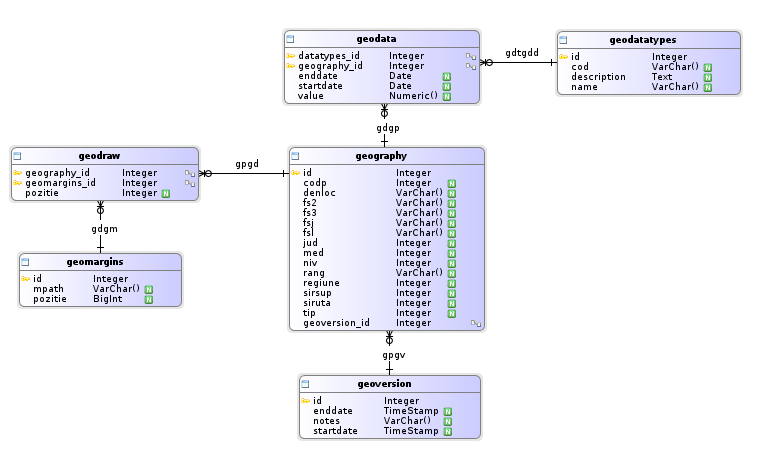
\includegraphics[width=\textwidth]{img/geo-database}

\subsubsection{Sistemul de vizualizare a hartilor}

Sistemul de vizualizare a hartilor este similar cu sistemul de vizualizare a datelor. Este construit pe baza aceleiasi biblioteci ExtJS. Este compus din doua panouri, unul de selectie a datelor si un altul de vizualizare a acestora. 

Panoul de selectie contine o structura arborescenta in care se pot vedea toti indicatorii disponibili si versiunile anuale ale acestora. 

Panoul de vizualizare a datelor contine o bara de instrumente in partea de sus si o componenta special pentru desen vectorial in partea de jos. 

Componenta pentru desen este bazat pe o librarie numita Raphael\footnote{\url{http://raphaeljs.com/}} care a fost integrata in ExtJS 4.0 si care permite desenul vectorial direct in paginile web. 
Componenta pentru desen se adapteaza automat la programul de navigare utilizat. in majoritatea browserelor moderne datele vor fi prezentate sub forma de SVG. 

Managerul de layout din ExtJS va dimensiona componenta de desenare in functie de containerul in care se afla. 
Odata desenat insa, acesta va ramane fix pana la redimensionarea ferestrei. 
Desenul din interiorul componentei va fi redimensionat separat de container pentru a putea fi observat la diferite nivele de marire. 

In interiorul componentei de desen se gaseste un ansamblu de poligoane, fiecare poligon reprezentand o unitate administrativa. 
Culoarea acestuia este calculata in functie de parametri pe care harta trebuie sa ii reprezinte. 
Fiecare poligon are declarat pe el trei evenimente:

\begin{itemize}
\item
mouse in (la intrarea cursorului mouse-ului pe suprafata poligonului) - creste grosimea granitelor poligonului
\item
mouse out (iesirea cursorului mouse-ului de pe suprafata poligonului) - scade grosimea granitelor poligonului
\item
click - se deschide o fereastra in care sune afisate detalii cu privire la unitatea administrativa respectiva
\end{itemize}

La incarcarea fiecarei harti se investigheaza daca aceasta are mai multe nivele de agregare. 
Daca da, in toolbar se va afisa un meniu care ofera posibilitatea incarcarii fiecarui nivel in parte. 
Componenta va afisa nivelul de agregare predefinit. 

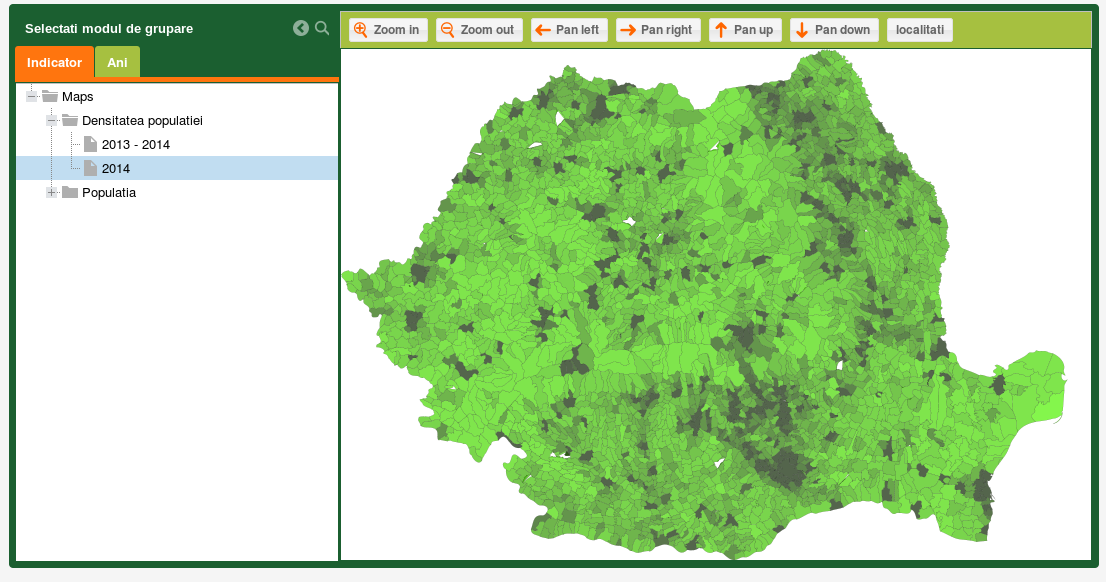
\includegraphics[width=\textwidth]{img/geo-map}

\subsubsection{Implementarea server-side a hartilor si datelor agregate}

Informatia referitoare la datele geografice si indicatorii pentru fiecare unitate teritoriala sunt stocate in baza de date, conform modelului de date descris anterior. 

Pe de o parte, introducerea acestor date in aplicatie a presupune crearea unor noi clase in partea de domeniu din arhitectura proiectului. 
Pe de alta parte, pentru ca aceste informatii sa fie disponibile in aplicatie, a fost necesara dezvoltarea unor noi clase de servicii si controller-e pe partea de server. 
Controller-ele sunt invocate prin intermediul unor URL-uri, 
alcatuite din sirul de caractere ce reprezinta contextul aplicatiei la care se adauga fragmentul corespunzator cererii respective. 
Acest fragment poate fi:
\begin{itemize}
\item
/geoversionslist - furnizeaza lista versiunilor referitoare la datele geografice disponibile. In interfata de administrare, aceste versiuni vor fi incarcate intr-o zona in care va fi posibila selectia.
\item
/geographybyversion/<version\_id> - permite obtinerea denumirilor unitatilor teritoriale pentru o versiune al carei identificator este specificat in URL. In interfata de administrare, aceste informatii vor corespunde versiunii selectate; la randul lor, vor fi disponibile pentru a fi selectate. 
\item
/geoindicatorlist/<geography\_id> - furnizeaza indicatorii existenti pentru o anumita zona geografica, specificata prin identificatorul sau. In interfata de administrare, aceste informatii vor corespunde unitatii teritoriale selectate.
\item
/geoindicatorvalues/<geography\_id>/<indicator> - permite obtinerea valorii unui indicator in cadrul unei unitati teritoriale. In interfata de administrare aceste informatii vor fi afisate pentru un indicator si o unitate teritoriala selectata.
\item
/geoborders/<geography\_id> - furnizeaza vectorul complet ce descrie intreaga margine a unei unitati teritoriale, prin compunerea tuturor marginilor stocate in baza de date. 
\end{itemize}
Acest ultim controller este util crearii dinamice a hartii in cadrul unei noi pagini a aplicatiei. Pentru aceasta, a fost definit un nou cod ce poate aparea in componentele corespunzatoare sistemului de management al continutului (CMS). 

\clearpage

\section{Rezultate, stadiul realiz\u{a}rii obiectivului, concluzii si propuneri pentru continuarea proiectului}

%TODO de completat la fiecare faza ???


\medskip


%\clearpage

\bigskip

\bigskip

\bigskip

\bigskip

\bigskip

\bigskip

\bigskip

\bigskip

{\bfseries
RECTOR,}

prof.univ.dr. Mircea Dumitru

\bigskip

\bigskip

\bigskip

\bigskip

\bigskip

\bigskip

\bigskip

\bigskip

{\bfseries
DIRECTOR GENERAL ADMINISTRATIV,}

ec. Adrian Albu

\bigskip

\bigskip

\bigskip

\bigskip

\bigskip

\bigskip

\bigskip

\bigskip

{\bfseries
RESPONSABIL PROIECT,}

lect.univ.dr. Adrian Du\c{s}a

\end{document}
